\section{Requerimientos funcionales}
A continuación, se presenta un listado con los requerimientos funcionales que se obtuvieron.
El listado de requerimientos funcionales se encuentra dividido de acuerdo con los módulos que se identificaron.

\paragraph{}
\begin{figure}[H]
	\centering
	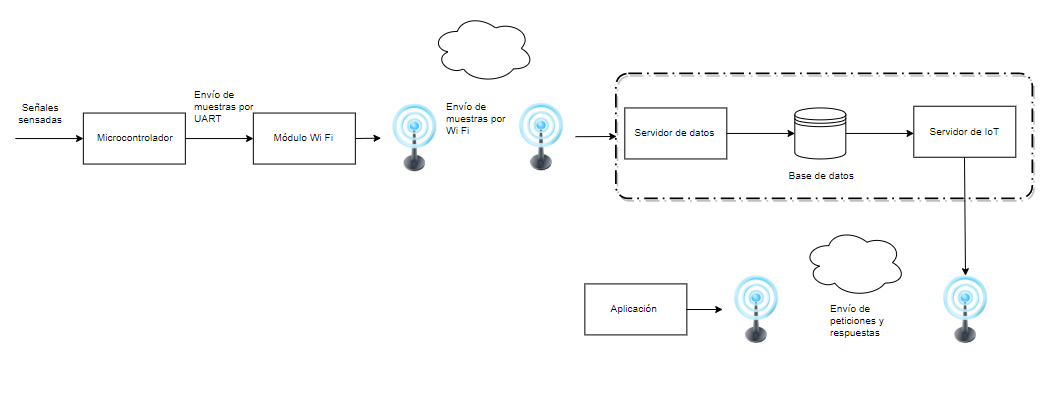
\includegraphics[scale=.3]{Capitulo3/img/diagramaBloques.png}
	\caption{Diagrama a bloques del sistema}
	\label{fig:diagrama_dispMonitoreo}
\end{figure}

\begin{itemize}
	\item Módulo de Microcontrolador.
	\item Módulo de Servidor.
	\item Módulo de Aplicación de usuario.
\end{itemize}

\paragraph{Módulo de Microcontrolador}
\begin{enumerate}[label=RF\arabic*.]
	\item Proporcionar un mecanismo de comunicación vía IIC desde el transductor MCP39F521 hacia el microcontrolador DSPIC30F4013.
	\item Proporcionar un mecanismo de comunicación vía UART desde el microcontrolador DSPIC30F4013 hacia el módulo Wi-Fi MIKROE-2542.
\end{enumerate}

\paragraph{Módulo de Servidor.}
\begin{enumerate}[label=RF\arabic*.]
	\setcounter{enumi}{2}
	\item Proporcionar un servicio para la recepción de los paquetes enviados por el módulo Wi-Fi MIKROE-2542 y su almacenamiento en un archivo de formato de texto.
	\item Proporcionar un servicio de comunicación vía HTTP para el envío de la información almacenada para dar respuesta a las peticiones realizadas por el usuario desde la aplicación móvil.  
\end{enumerate}

\paragraph{Módulo de Aplicación de usuario.}
\begin{enumerate}[label=RF\arabic*.]
	\setcounter{enumi}{4}
	\item Proporcionar un mecanismo para la vinculación entre la aplicación y el servidor.
	\item Proporcionar un servicio de comunicación vía HTTP para la generación de peticiones al servidor.
	\item Proporcionar un mecanismo para la visualización en tiempo real de la generación  de la energía producida por el sistema fotovoltaico.
	\item Proporcionar un mecanismo para la generación de estadísticas de la producción de energía por el sistema fotovoltaico.
	\item Informar por medio de notificaciones cuando el sistema fotovoltaico dejó de producir energía, así como al final del día notificar si se produjo más o menos energía que el promedio diario de producción.  
\end{enumerate}